\documentclass[10pt]{beamer}

\usepackage[utf8]{inputenc}
\usepackage[spanish]{babel}

\usepackage{graphicx}
\graphicspath{./Multimedia/}
\usepackage{multimedia}

\usepackage{hyperref}

\usetheme[progressbar=frametitle]{metropolis}
\usepackage{appendixnumberbeamer}

\usepackage{booktabs}
\usepackage[scale=2]{ccicons}

\usepackage{pgfplots}
\usepgfplotslibrary{dateplot}

\usepackage{xspace}

\title{Tor, ¿la herramienta definitiva de anonimato?}
\date{}
\author{Ignacio Aguilera Martos}
\titlegraphic{Interferencias\hfill\includegraphics[height=1.5cm]{./Multimedia/interferencias.jpg}}


\begin{document}
	

	
	
%Diapositiva de Título.
\frame{\titlepage}

%%%%%%%%%%%%%%%%%%%%%%%%%%%%%%%%%%%%%%%%%%%%%%%%%%%%%%%%%%%%%%%%%%%%%%%%%%%%%%%%%%%%%%%%%
%%%%%%%%%%%%%%%%%%%%%%%%%%% Anonimato en la red con Tor %%%%%%%%%%%%%%%%%%%%%%%%%%%%%%%%%
%%%%%%%%%%%%%%%%%%%%%%%%%%%%%%%%%%%%%%%%%%%%%%%%%%%%%%%%%%%%%%%%%%%%%%%%%%%%%%%%%%%%%%%%%
	
%Índice
\begin{frame}{Contenidos}
	\setbeamertemplate{section in toc}[sections numbered]
	\tableofcontents[hideallsubsections]
\end{frame}

\begin{frame}{Licencia}
	\begin{center}
		GNU GENERAL PUBLIC LICENSE \\
		Version 3, 29 June 2007 \\
		
		Copyright (C) 2007 Free Software Foundation, Inc. http://fsf.org/ \\
		Everyone is permitted to copy and distribute verbatim copies \\
		of this license document, but changing it is not allowed.
	\end{center}
\centering	www.github.com/nacheteam/Charla-sobre-Tor
\end{frame}

%¿Qué es Interferencias?
\section{Interferencias}

\begin{frame}{Interferencias}
	\begin{block}{Interferencias}
		Interferencias es un grupo sin ánimo de lucro que pretende reunir a una serie de personas interesadas en:
		
		\begin{itemize}
			\item Privacidad
			\item Vigilancia masiva
			\item Derechos en internet
			\item Seguridad
		\end{itemize}
	\end{block}
	\begin{center}
		Twitter: @Inter\_ferencias \\
		E-mail: interferencias@protonmail.com \\
		interferencias.github.io
	\end{center}
\end{frame}

%Sección de introducción al anonimato
\section{¿Por qué es importante el anonimato?}

\begin{frame}{Anonimato}
	\begin{itemize}
		\item Debemos ser dueños de nuestra información. \pause
		\item No somos manipulados en función de nuestros datos si permanecemos anónimos. \pause
	\end{itemize}
	\metroset{block=fill}
	\begin{block}{Privacidad en Internet}
		\pause La privacidad en Internet se refiere al derecho de la privacidad personal en relación con el almacenamiento, la reutilización, la provisión a terceros y la exhibición de información relativa a uno mismo a través de Internet.
	\end{block}
	\pause
	\begin{alertblock}{Charla de Introducción a la privacidad}
		$https://bitbucket.org/josealberto4444/charla\_introduccion\_privacidad$
	\end{alertblock}
\end{frame}


%Sección que se incluye en el índice.
\section{Tor(The onion router)}

%Diapositiva de introducción de Tor.
\begin{frame}[fragile]{Propósito de Tor}
	%Lista de cosas que aparecen en diferentes páginas.
	\begin{itemize}
		\item<1-> Comunicaciones anónimas.
		\item<2-> $\boldsymbol{NO}$ se pretende respaldar a delincuentes.
		\item<3-> Es una red compleja de analizar.
	\end{itemize}
\end{frame}

%Diapositiva del esquema básico de Tor
\begin{frame}[fragile]{Esquema básico de Tor}
	\pause
	Las entidades básicas de Tor son:\pause
	\begin{itemize}
		\item<1-> Nodos.\pause
		\item<2-> Usuarios.\pause
		\item<3-> Autoridades de Directorio.
	\end{itemize}
	\pause
	\metroset{block=fill}
	%Bloque de alerta de información.
	\begin{alertblock}{Proxys y Tor}
		La relación entre nodos es similar a los proxys pero no es la misma.
	\end{alertblock}
\end{frame}

%Diapositiva acerca de los nodos.
\begin{frame}[fragile]{Nodos y sus tipos}
	\pause
	Los nodos son las piezas fundamentales de Tor.\\
	\pause
	Tipos: \pause
	\metroset{block=fill}
	%Bloque de definición.
	\begin{block}{Nodos Guard o Nodos de entrada}
		Son los nodos que ocupan el primer lugar en los circuitos. Son críticos ya que conocen la identidad del usuario.
	\end{block}
	\pause
	\begin{block}{Middle Nodes o Relay}
		Son los nodos intermedios dentro de los circuitos. Son los más básicos.
	\end{block}
	\pause
	\begin{block}{Exit Nodes o Nodos de salida}
		Son los nodos que ocupan el último lugar de los circuitos. Estos nodos tienen la información sin encriptar para enviarla al servidor de destino.
	\end{block}
\end{frame}

%Diapositiva acerca de los circuitos.
\begin{frame}[fragile]{Circuitos y su temporalidad}
	\pause
	\metroset{block=fill}
	\begin{block}{Circuito}
		Es un camino de nodos dentro del grafo de la red Tor. Incluye un nodo de entrada, varios nodos intermedios y un nodo de salida.
	\end{block}
	\pause
	Los circuitos tienen una caducidad (modificable por el usuario) por motivos de seguridad.
\end{frame}

%Diapositiva sobre los flags de los nodos.
\begin{frame}[fragile]{Flags de calificación de nodos}
	\pause
	\begin{itemize}
		\item<1-> BadExit.\pause
		\item<2-> Fast : 100KB/s.\pause
		\item<3-> Guard: 250KB/s. \pause
		\item<4-> Authority.\pause
		\item<5-> Exit.\pause
		\item<6-> HSDir: Hidden Service Directory.\pause
		\item<7-> Named o Unnamed.\pause
		\item<8-> Running: 45 minutos en ejecución.\pause
		\item<9-> Stable: 7 días en ejecución.\pause
		\item<10-> Valid: lista negra y versión de Tor sin alterar.\pause
		\item<11-> V2Dir\pause
	\end{itemize}
	\pause
	Gracias a estos flags los nodos quedan valorados para saber su posición en los circuitos y su validez como nodo en general.
\end{frame}

%Diapositiva acerca del ciclo de vida de un nodo.
\begin{frame}[fragile]{Ciclo de vida de un nodo}
	\pause
	Ocurre en 4 fases:
	\pause
	\begin{itemize}
		\item<1-> Fase 1(0-3): Comprobaciones básicas. Tests de seguridad y velocidad.\pause
		\item<2-> Fase 2(3-8): Nodo intermedio. Comprobaciones sobre Guard y Exit.\pause
		\item<3-> Fase 3(8-68): Nodo Guard. Comprobaciones de estabilidad y Exit.\pause
		\item<4-> Fase 4(68-...): Nodo Exit. Comprobaciones esporádicas generales.\pause
	\end{itemize}
\end{frame}

%Diapositiva sobre los servicios ocultos.
\begin{frame}[fragile]{Servicios Ocultos}
	\pause
	Los integrantes de esta comunicación son:
	\pause
	\begin{itemize}
		\item<1-> Usuario.\pause
		\item<2-> Servicio Oculto.\pause
		\item<3-> Puntos Introductorios.\pause
		\item<4-> Nodo Rendezvous.\pause
	\end{itemize}
	\pause
	\metroset{block=fill}
	\begin{block}{Diagrama de Comunicación}
		\footnotesize $Usuario \Leftrightarrow Guard \Leftrightarrow Relay \Leftrightarrow Rendezvous \Leftrightarrow Relay \Leftrightarrow Guard \Leftrightarrow Servicio \ oculto$
	\end{block}
	\pause
	\begin{exampleblock}{Direcciones Onion}
		Los servicios ocultos tienen URLs con el dominio onion y contienen 16 caracteres.\\ Por ejemplo: ab2dafgh6jklmi3t.onion ó facebookcorewwwi.onion.
		Deben ser caracteres entre la 'a' y la 'z' y números entre el '2' y el '7'.
	\end{exampleblock}
\end{frame}

%Diapositiva de Descriptores
\begin{frame}[fragile]{Descriptores}
	\pause
	\begin{itemize}
		\item<1-> Server Descriptor: IP, ORPort, ... \pause
		\item<2-> ExtraInfo Descriptor: Información completa del nodo. \pause
		\item<3-> Micro Descriptor: Información reducida del nodo. \pause
		\item<4-> Network Status Document: fichero de consenso.\pause
		\item<5-> Router Status Entry: Información completa de nodos incluyendo flags y cálculos heurísticos.\pause
		\item<6-> Hidden Service Descriptor: Información del servicio oculto.\pause
	\end{itemize}
\end{frame}

%Diapositiva de Puentes
\begin{frame}[fragile]{Puentes}
	\pause
	\metroset{block=fill}
	\begin{block}{Puente}
		Nodos ocultos usados para impedir las prohibiciones de uso de Tor por gobiernos o cualquier otra entidad.
	\end{block}
\end{frame}

%Diapositiva de Autoridades de Directorio.
\begin{frame}[fragile]{Autoridades de Directorio}
	\pause
	\metroset{block=fill}
	\begin{block}{Autoridad de Directorio}
		Nodo con permisos totales en la red. Son los únicos nodos de confianza. Tienen como misión controlar los nodos, valorarlos y administrar la red en general.
	\end{block}
\end{frame}

%Diapositiva de los ataque a Tor.
\begin{frame}[fragile]{Vulnerabilidades y fallos de diseño}
	\pause
	\metroset{block=fill}
	\begin{itemize}
		\item<1-> Correlación punto a punto.\pause
		\item<2-> Pérdida de información del nodo de salida.\pause
		\item<3-> Bloqueo de los nodos de salida.\pause
		\item<4-> Ataque DDOS a Tor.\pause
		\item<5-> HeartBleed.\pause
		\item<6-> DNS Leak.\pause
		\item<7-> Clogging(Saturación de nodos).\pause
		\item<8-> Round Trip Travel Time.\pause
	\end{itemize}
\end{frame}

%Sección del Tor Browser
\section{Tor Browser}

%Cómo descargar y configurar el Tor Browser.
\begin{frame}{¿Cómo obtener el Tor Browser?}
	\pause
	\metroset{block=fill}
	\begin{block}{Tor Project}
		www.torproject.org
	\end{block}
	
	\begin{figure}
		\centering
		\href{http://www.torproject.org}{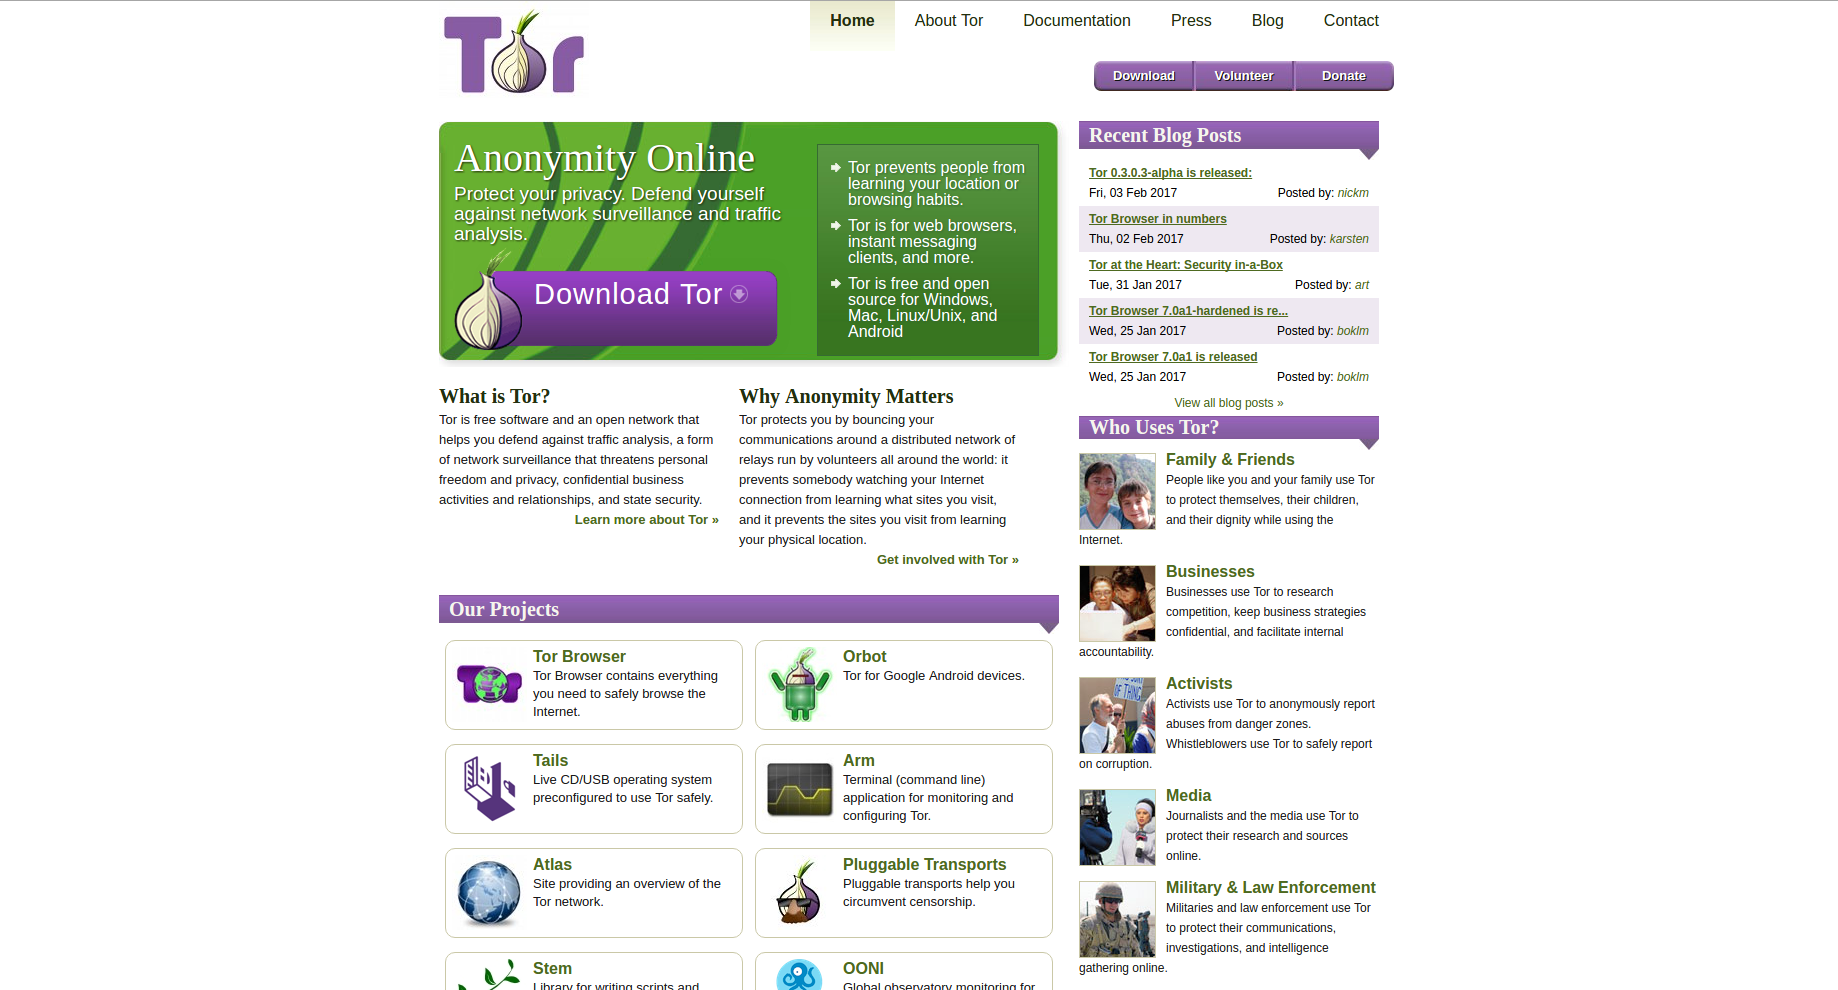
\includegraphics[scale=0.15]{./Multimedia/tor_project.png}}
	\end{figure}
\end{frame}

\begin{frame}{Buenas Prácticas con Tor}
	\begin{itemize}
		\item<1-> Utilizar el Tor Browser para navegar por Internet.\pause
		\item<2-> Utilizar Tails.\pause
		\item<3-> Navegar por webs https siempre que sea posible.\pause
		\item<4-> No introducir credenciales salvo en webs https.\pause
		\item<5-> No montar un nodo de salida si no sabes cómo hacerlo bien.\pause
	\end{itemize}
	\metroset{block=fill}
	\begin{alertblock}{Facebook no es tu amigo}
		Aunque Facebook tenga su web en Tor (facebookcorewwwi.onion) no lo hagáis...
	\end{alertblock}
\end{frame}

\section{Enlaces de Interés}

\begin{frame}{Tor flow}
	\pause
	\metroset{block=fill}
	\begin{block}{Tor flow}
		Tor flow es una web que muestra información del tráfico de la red Tor sobre un mapa del mundo interactivo.
	\end{block}
	\pause
	\centering\href{http://torflow.uncharted.software}{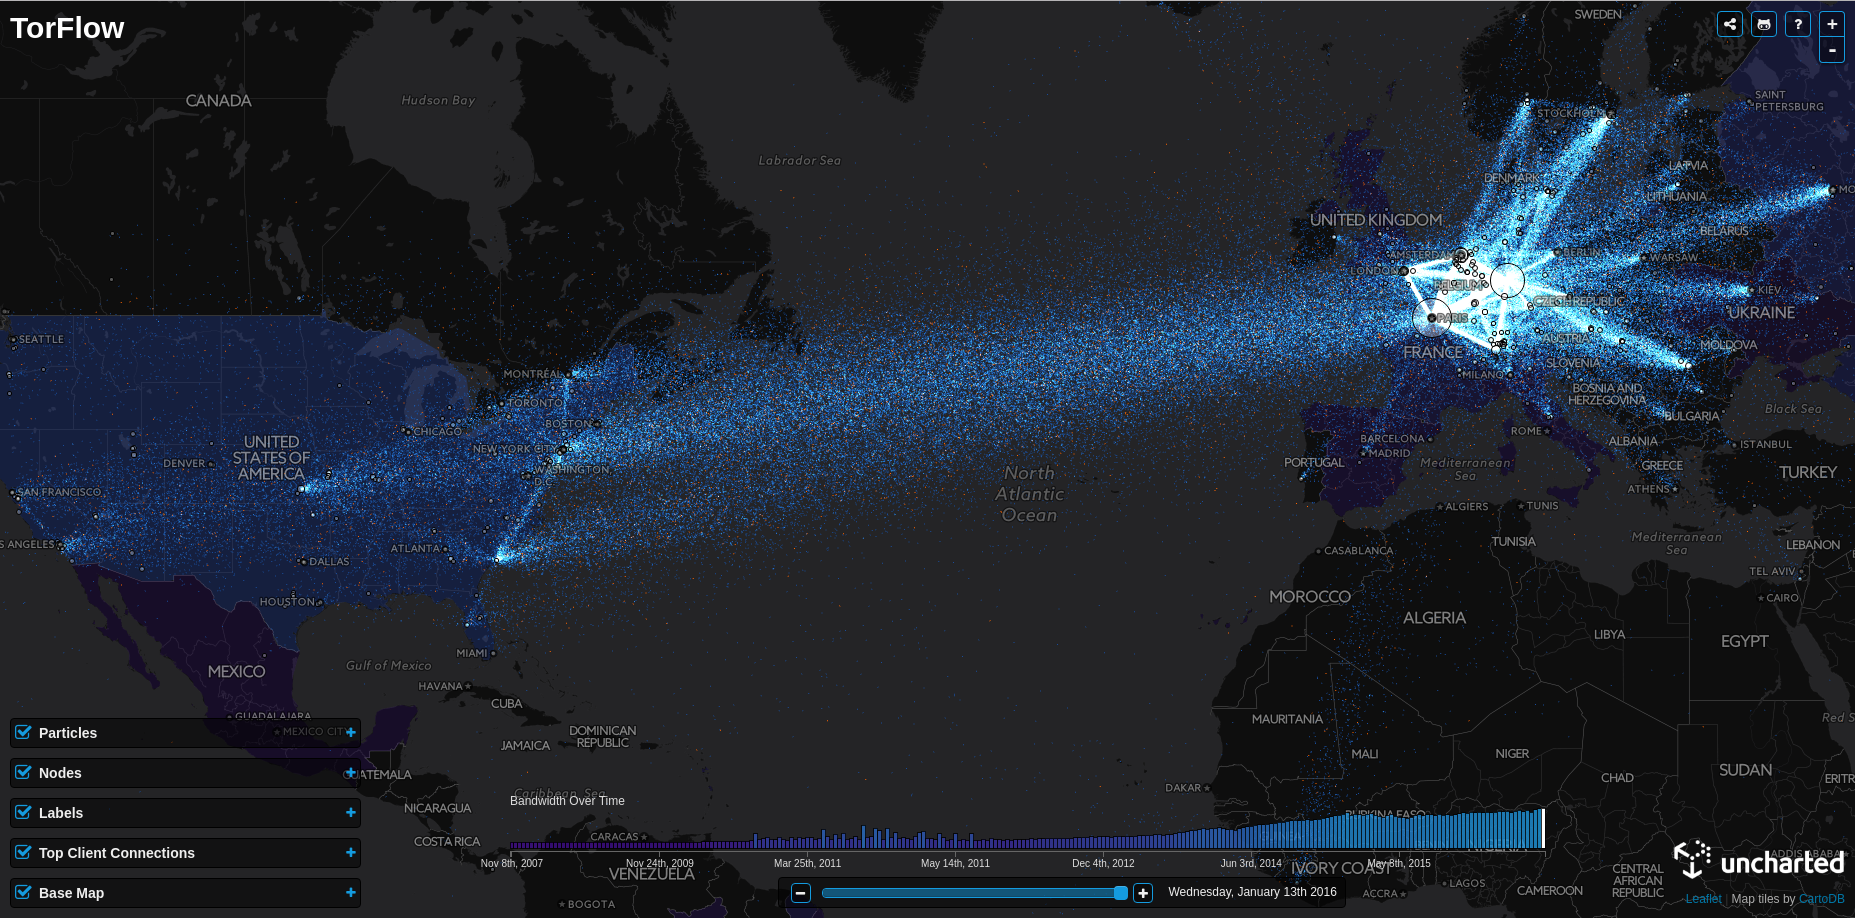
\includegraphics[scale=0.1]{./Multimedia/tor_flow.png}}
\end{frame}

\begin{frame}{Tor metrics}
	\pause
	\metroset{block=fill}
	\begin{block}{Tor Metrics}
		Tor metrics es una web que nos da información estadística acerca de la red tor.
	\end{block}
	\pause
%	\centering\href{https://metrics.torproject.org}{\includegraphics[scale=0.1]{./Multimedia/}}
\end{frame}

\begin{frame}[standout]
	\centering ¿Preguntas? \\ 
	
	\begin{center}
		\includegraphics[scale=0.1]{./Multimedia/interferencias.jpg}
	\end{center}
\end{frame}
	
\end{document}